\chapter{Introdução}
Tendo em vista a necessidade de aspiração em piscinas e a crescente onda de automação residencial, observou-se a oportunidade de produzir um equipamento para realizar tal tarefa automática de piscinas (Kanno et al, 2014).

Considerando o alto custo de aquisição de equipamentos modernos, internacionais e a grande demanda por serviços de higienização de piscinas, e o fato de que no Brasil não há empresas que desenvolvam este produto (há apenas revendedoras), o desenvolvimento do Clean Pool Robot permitirá a aplicação do conceito de automação a ambientes residenciais e a redução dos gastos com a contratação de um serviço terceirizado. As principais vantagens na utilização do Clean Pool Robot são:

\begin{itemize}
\item Retirar detritos do fundo da piscina que não foram alcançados por outros meios;
\item Mover a água ao passo que limpa as superfícies, melhorando a sua circulação;
\item Produzir um produto nacional que possui valor de mercado mais acessível.
\end{itemize}

Em uma pesquisa realizada pela equipe, verificou-se que a massa dos robôs que limpam piscinas variam de 8 Kg até 25 Kg e custam entre R\$ 2.000,00 e R\$ 16.000,00. O \cpr tem massa de aproximadamente 10kg e custará em torno de R\$ 7.000,00, preço mediano entre os concorrentes. Para a escolha de um limpador de piscinas automático, pequenas diferenças de especificação devem ser consideradas no momento da aquisição do aparelho, como por exemplo, ciclo de limpeza e taxa de filtragem. O ciclo de limpeza determina o intervalo de tempo em que o robô trabalha antes de se desligar automaticamente e a taxa de filtragem é determinada pela quantidade de água filtrada em uma hora, que é expressa em litros por hora (LPH). No caso do CPR tem um ciclo de limpeza de 5h, tempo necessário para limpar uma piscina curta (semiolímpica).

O \cpr estará lidando basicamente com um corpo imerso em um líquido. Deste modo, o corpo estará essencialmente sob ação de duas forças: empuxo e peso.  Empuxo ocorre quando um corpo imerso na água parece ter se tornado mais leve devido a uma força, exercida pelo líquido sobre o corpo, vertical e para cima, que alivia o peso do corpo. Já o peso é devido à interação com o campo gravitacional da Terra.

Quando um corpo está totalmente imerso em um líquido, podemos ter as seguintes situações: 

\begin{itemize}
\item Se ele permanecer parado no ponto onde foi colocado, a intensidade da força de empuxo é igual à intensidade da força peso;
\item Se ele afundar, a intensidade da força de empuxo é menor do que a intensidade da força peso;
\item Se ele for levado para a superfície, à intensidade da força de empuxo é maior do que a intensidade da força peso.
\end{itemize}

Como o robô realiza a limpeza do fundo da piscina, este deve estar afundado, ou seja, a intensidade da força de empuxo deverá ser menor do que a intensidade da força peso.

\section{Objetivos do Projeto}
Construir um robô capaz de realizar a remoção de sujeiras depositadas no fundo de piscinas por meio da aspiração e filtragem das impurezas. Os objetivos específicos são:

\begin{itemize}
\item Realizar aspiração automática dos resíduos decantados por meio da sucção e filtragem;
\item Submergir de forma independente;
\item Movimentar-se ao longo do fundo da piscina.
\end{itemize}

\section{Estrutura do Relatório}
A organização do projeto foi dividido em dois grupos: o grupo de estrutura e o grupo de lógica. Ambos os grupos se relacionam e tem trabalhado em conjunto. O diagrama abaixo apresenta a interação entre os grupos e as diversas engenharias que os compõem.
\par
  \begin{figure}[h]
    \centering
    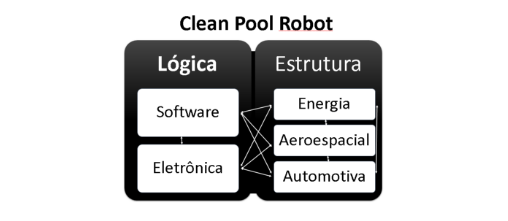
\includegraphics[width=0.8\textwidth]{figures/technical-div-project.png}
    \caption{Divisão técnica do projeto em dois segmentos.}
    \label{fig:technical-div-project}
  \end{figure}
  \FloatBarrier
\par
Apesar da divisão em duas grandes equipes, os membros interagiram de forma a preencher os requisitos e parâmetros solicitados por meio de documentos compartilhados via Google drive, ou por mensagens em grupos de conversa privados, utilizando-se do \textsf{WhatsApp}.

Nos próximos itens do relatório estão a visão geral no nosso produto, onde apresenta-se o \textit{design}, os sistemas que o compõem, os indicadores e a estimativa de custo. Em seguida tem-se o dimensionamento de cada componente. Por fim, a montagem do protótipo e os testes realizados.

\chapter{O \textit{Clean Pool Robot}}
\section{Visão Geral}
O \cpr é um equipamento que visa auxiliar a limpeza de grandes piscinas, como os modelos semiolímpicos. O robô faz a aspiração e filtragem das impurezas presentes no fundo da piscina, removendo as algas e folhas e auxiliando na circulação da água. O mecanismo do mesmo será composto por dois métodos para que o fundo da piscina possa ser aspirado: o primeiro baseia-se na escovação do chão e o segundo a sucção das impurezas desprendidas do piso da piscina.

O primeiro método tem foco nas escovas que estão situadas na parte inferior do robô. As escovas realizam movimentos giratórios fazendo com que suas cerdas entrem em contato com o chão retirando  impurezas, como por exemplo: algas e grãos de terra.

Após a escovação, é realizado outro método, a sucção das impurezas desprendidas do piso da piscina  além de outras impurezas que estiverem próximas à área de atuação do robô, por exemplo: pequenos ramos e folhas. Por meio de uma bomba, a água é sugada por uma abertura situada na parte inferior e passa por um filtro. As impurezas menores ficam retidas no filtro. Por meio de um sistema de expulsão de água, esta sairá a uma velocidade muito superior à velocidade de entrada no início do processo, ajudando na movimentação do robô.

Com o término da limpeza na piscina, haverá a necessidade dos filtros serem limpos para retirada das impurezas colhidas na aspiração da água. Assim, após cada utilização o usuário deverá limpar os filtros internos do \cpr.

O produto desenvolvido será responsável apenas pela retirada da sujeira decantada no fundo da piscina, ou seja, o \cpr não limpará as paredes ou superfície da piscina. Além disso, as piscinas ideais para a operação do robô são as retangulares, sem inclinações e azulejadas. É ideal também que o robô seja lançado na piscina no meio da largura maior, evitando que o fio fique totalmente esticado quando o robô estiver na quina oposta do lançamento.  

\section{O \textit{Design}}
A Figura \ref{fig:croqui-design-cpr} mostra o \cpr projetado no \software Catia. O modelo apresenta dois rolos de limpeza, localizados na parte frontal e traseira do robô, um duto, na parte superior para a saída da água filtrada, que também funciona como propulsão e direcionador dos movimentos do robô. A sucção da água feita por meio das duas aberturas na parte inferior do robô. Abaixo a figura com croqui do design do \textit{Clean Pool Robot}.
\par
  \begin{figure}[h]
    \centering
    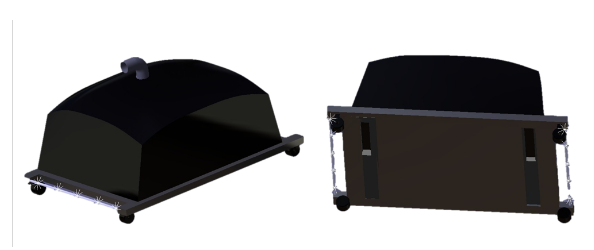
\includegraphics[width=0.8\textwidth]{figures/croqui-design-cpr.png}
    \caption{Croqui com o design do \textit{Clean Pool Robot}, vista frontal e inferior.}
    \label{fig:croqui-design-cpr}
  \end{figure}
  \FloatBarrier
\par
Por motivo de resistência ao movimento o formato do robô foi modificado para melhor aproveitamento das forças hidrodinâmica envolvidas, as alterações no desenho inicial foram feitas com a intenção de diminuir a força de arrasto, a estrutura conta agora com cantos e arestas arredondadas conforme a Figura \ref{fig:croqui-design-cpr}.

O \textit{design} apresentado é a segunda versão, em que foi melhorado o posicionamento das escovas. Nessa versão elas ficam na extremidade do robô, onde auxiliam em eventuais impactos (por mais que seja pequeno) do robô com a parede.

\section{Sistemas}
O Robô possui três principais sistemas para o seu funcionamento: o Sistema de Automação, composto pelos sensores e programações lógicas de acionamento, Sistema de Locomoção, formado pelo conjunto das rodas, bomba e motores, e o Sistema de Limpeza, com os filtros e rolos de limpeza. A Figura \ref{fig:main-system-project} mostra os três sistemas e a relação entre eles.
\par
  \begin{figure}[h]
    \centering
    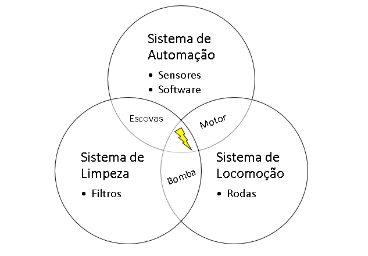
\includegraphics[width=0.8\textwidth]{figures/main-system-project.png}
    \caption{Três principais sistemas do Robô: Automação, Limpeza e Locomoção.}
    \label{fig:main-system-project}
  \end{figure}
  \FloatBarrier
\par

\section{Indicadores}
Os indicadores de desempenho são métricas que quantificam a performance de acordo com os objetivos propostos. Para auxiliar a validação da verificação da limpeza do robô, determinou-se um indicador que é o \textsf{CDL} - Ciclo de Limpeza.

O \textsf{CDL} faz uma avaliação da limpeza em gruas de leve até uma limpeza minuciosa. O parâmetro para a avaliação do cliclo se faz em comparação com tempo, caso a duração total da limpeza seja menor que 5h, então o robô terá executado um \textsf{CDL} leve, ou seja, limpeza rápida e mais leve. Esse \textsf{CDL} é indicado para piscinas que estejam, por inspeção visual, com pouca sujeita depositada ao fundo.

Caso o tempo total da limpeza seja maior que 5h, o \textsf{CDL} utilizado foi equivalente a uma limpeza minuciosa. Neste caso a piscina deve estar com maior quantidade de impurezas depositadas ao fundo. A Figura \ref{fig:indicator} mostra a represenatção do indicador.
\par
  \begin{figure}[h]
    \centering
    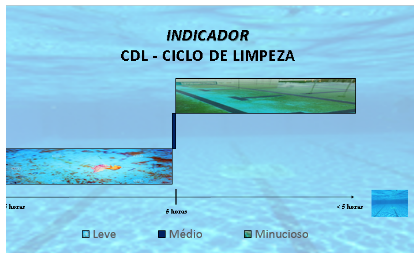
\includegraphics[width=0.8\textwidth]{figures/indicator.png}
    \caption{Indicador CDL.}
    \label{fig:indicator}
  \end{figure}
  \FloatBarrier
\par

\section{Custos}
No desenvolvimento do \cpr foram gastos até o momento os valores apresentados na tabela abaixo. Considerando um lucro de 10\% sob cada peça, o custo estimado para a venda do Robô é de R\$ 6.500, estando comercialmente competitivo.
\begin{table}[h]
\centering
\caption{Valores de Custos do \textit{Clean Pool Robot}}
\label{my-label}
\begin{tabular}{@{}cc@{}}
Carga horária máxima                      & 90 h         \\
Valor da Hora (Valor da Capes – Graduado) & R\$ 24, 44   \\
Pessoas no desenvolvimento do produto     & 12           \\
Hora por mês                              & 20           \\
Preço total da mão de obra                & R\$ 5.866,67 \\
Material                                  & R\$ 1.349,50 \\
Lucro                                     & 10\%         \\ \midrule
Valor total para Venda (sem impostos)     & R\$ 6.494,55
\end{tabular}
\end{table}

Uma pesquisa realizada apresentou o custo dos principais concorrentes do Clean Pool Robot que está entre R\$ 2.000,00 e R\$ 16.000,00, assim o valor de mercado está dentro da classe dos produtos mais baratos.

\chapter{Sistemas do Robô}
\section{O Sistema de Locomoção}
\subsection{Duto de Propulsão}
A água que é ejetada do sistema de filtragem é devolvida para a piscina, auxiliando assim a limpeza geral de todo o volume em que o robô está submerso. A água filtrada é direcionada para uma saída que se localiza na parte superior do produto. O duto de saída será um bocal direcionável localizado na parte superior do robô responsável por sua locomoção. Esse bocal irá se mover nas 4 direções principais, isto é, nos ângulos de 0, 90, 180 e 270 graus, proporcionando ao robô a locomoção necessária para o cumprimento da rota de limpeza.

O duto de propulsão terá diametro de 1” (25,4mm). Acoplado a ele está o propulsor auxiliar que permitirá a movimentação do robô com a velocidade desejada. O duto de propulsão foi construído de forma que a água mude de direção sem que haja vazamentos e que o servo responsável pela rotação não entre em contato com a água.

\subsection{As Rodas}
O aparelho contará com quatro rodas. Elas se assemelham as usadas em carrinhos de supermercado, com liberdade de 360 graus em relação ao eixo $x$ e $y$.
\par
  \begin{figure}[h]
    \centering
    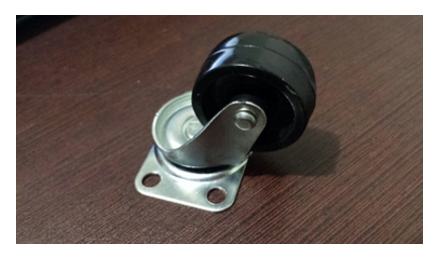
\includegraphics[width=0.6\textwidth]{figures/wheel-market.png}
    \caption{Rodas utilizadas para a locomoção do robô.}
    \label{fig:wheel-market}
  \end{figure}
  \FloatBarrier
\par
As rodas serão fixadas na placa da base do robô e estarão localizadas nos cantos da base do robô e direcionarão o seu movimento de acordo com a direção do jato de água oriundo do bocal, conforme a Figura \ref{fig:catia-base}.
\par
  \begin{figure}[h]
    \centering
    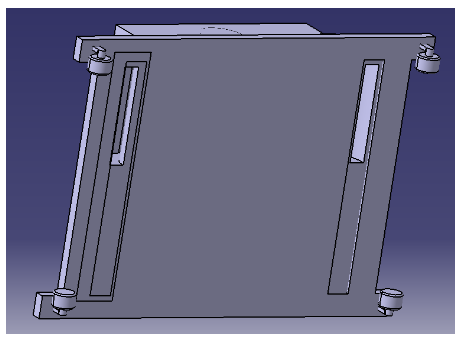
\includegraphics[width=0.8\textwidth]{figures/catia-base.png}
    \caption{Desenho da base do robô indicando as posições das rodas.}
    \label{fig:catia-base}
  \end{figure}
  \FloatBarrier
\par

\section{O Sistema de Limpeza}
\subsection{Os Filtros}
A filtragem irá garantir que a piscina estará limpa após o uso do \textit{Clean Pool Robot}. O filtro será fundamental, pois ele será responsável pela remoção das partículas de sujeira que ficam decantadas no fundo da piscina. Primeiro a água será sugada para dentro do aparelho que passará por um depósito onde será feita a filtragem. Em seguida, a água filtrada retorna para piscina. Será realizado um sistema de dupla filtragem com dois tipos de elementos filtrantes: um de malha de alumínio, elemento secundário, para evitar que folhas e objetos de maior tamanho entrem no filtro principal que será responsável por filtrar o particulado e detritos da água.

Será usada uma malha de alumínio para a realização de uma pré-filtragem, a qual impedirá que folhas, plásticos, cabelos, e outros materiais maiores entupam o filtro principal responsável por retirar impurezas menores da água. Essa malha é o que chamou-se de filtro secundário. O filtro principal será um elemento filtrante na forma cilíndrica comumente utilizado na filtragem de caixas d’águas. As imagens dos filtros a serem utilizados e as especificações técnicas do elemento filtrante principal constam a seguir. Juntamente com o sistema de filtragem existe o que chamamos de “caixa de sujeira”, nela a pedras, folhas, galhos e outros objetos que poderam entupir ou diminuir a vazão de filtragem serão armazenadas. Essa caixa deverá ser limpa sempre que o robô for retrado da água.
\begin{description}
\item[Malha de Alumínio:] A malha de alumínio é um material durável, altamente resistente água, não precisa de manutenção e nem de troca. Em caso de avaria na grade a substituição é simples e barata. A grade será localizada na entrada da caixa filtradora, no duto de acesso na base do robô, conforme imagem abaixo.
\par
  \begin{figure}[h]
    \centering
    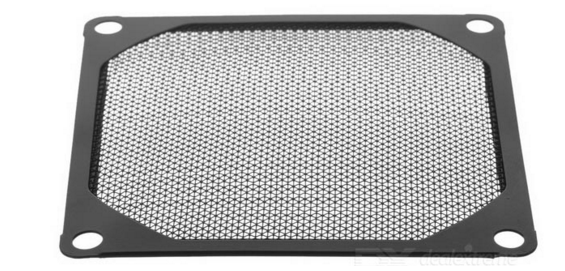
\includegraphics[width=0.8\textwidth]{figures/mesh-aluminium.png}
    \caption{Modelo de malha de alumínio utilizada como filtro secundário.}
    \label{fig:mesh-aluminium}
  \end{figure}
  \FloatBarrier
\par
\item[Elemento Filtrante:] as seguintes características são requeridas.

\begin{itemize}
\item Temperatura de operação: 5ºC mín. a 50ºC máx.
\item Vazão: 4.200 litros/hora
\item Grau de filtração: 50 micra (um grão de areia tem entre 200 a 500 micra)
\item Peso bruto: 448g
\item Peso líquido: 337g
\end{itemize}
Para se garantir a qualidade da água filtrada é indicado pelo fabricante a substituição dos elementos filtrantes Poly Flow a cada 6 meses ou quando for observada a redução do fluxo da água. O elemento filtrante é descartável, não necessita retrolavagem. A manutenção periódica do elemento é aconselhável. Para isso, utilize apenas água e uma escova macia.

Dimensões: Altura: 254mm; Diâmetro externo: 116mm; Diâmetro interno: 26mm.
\par
  \begin{figure}[h]
    \centering
    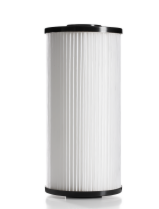
\includegraphics[width=0.2\textwidth]{figures/filter.png}
    \caption{Elemento Filtrante}
    \label{fig:filter}
  \end{figure}
  \FloatBarrier
\par
\end{description}
\subsection{O Dimensionamento dos Filtros}
Os filtros foram dimensionados, ou escolhidos, a partir dos pré-requisitos do projeto, isto é, velocidade, limpeza, area de atuação. Após a analise do que deveria ser filtrado e das possiveis fontes de entupimento do sistema de filtragem, dividiu-se o sistema em 3 áreas: caixa de sujeira; filtro secundario; filtro principal.

\subsection{Os Rolos de Limpeza}
Das principais sujeitas depositadas no fundo de piscinas pode-se listar: folhas e pequenos gravetos de arvores presentes nos arredores, além do acúmulo de algas, fungos e bactérias no fundo. Como solução para a limpeza destas sujeiras a utilização de peças com superficies mais macias ajudam a desgrudar do fundo as impurezas, independente de qual for o revestimento da piscina, se ele for azulejo, vinil, fibra ou pintura.(7)

Os rolos de limpeza estão localizados na parte frontal e traseira do robô, e  terão duas funções: a principal é auxiliar na remoção das impurezas do fundo da piscina, e a função secundária se dá no auxilio a sustentação do robô. 

Para o processo principal, a remoção das pequenas partículas depositadas no fundo da piscina, o rolo irá deslizar sob a superfície, sem que seja produzido muito atrito, para que não altere a velocidade total do robo e não danifique a superfície. Assim o material do rolo deve ser macio, leve e ao mesmo tempo resistente a água.

Para o processo secundário, de auxilio a sustentaçao do robô os rolos devem tem o seu raio na distância do fundo da piscina até a estrada de sucção, ou seja, a altura das rodas, pois assim o robô ficará nivelado e ao mesmo tempo com apoio na frente, atrás e no centro. Para esse requisito, o atendimento do design proposto, os rolos deverão ter, cada um deles, 300 mm de comprimento, 60 mm de diâmetro total e um eixo central com 30 mm de diâmetro, no qual será encaixado os eixos de rotação para os motores.

Definiu-se primeiramente utilizar escovas de formato cilíndrico e de Nylon, afim de que á medida que as rodas do robô se movem, as escovas também possam acompanhar o movimento sem maiores problemas. Porém a dificuldade em encontrar fabricantes e modelos em Brasilia e devido também ao elevado custo decidiu-se pela fabricação das escovas. Para a fabricação usou-se um tubo 50 mm de pvc e um revestimento de polimero, a fibra de vinil. 

A utlização de um polímero possui várias vantagens, tais como: baixa densidade, alta resistência à corrosão, baixo custo de aquisição, coeficiente de atrito baixo e grande flexibilidade. O baixo custo e densidade foram os principais motivos para a realização da troca.
\par
  \begin{figure}[h]
    \centering
    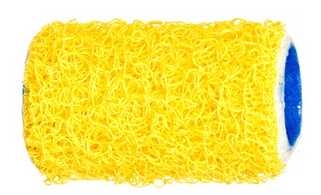
\includegraphics[width=0.5\textwidth]{figures/brush-vinil.png}
    \caption{Rolo de fibra de vinil.}
    \label{fig:brush-vinil}
  \end{figure}
  \FloatBarrier
\par

\section{Os Motores}
Serão utilizados dois motores elétricos para rotacionar os rolos de limpeza. A transmissão do torque para os rolos será por engrenagens. O modelo de motor a ser usado é o: Micro Motor DC 12V 18200RPM 390.40Gf.cm que possui as seguintes especificações:

Especificações técnicas do produto:
\begin{itemize}
\item Corrente: 1350,00 mA;
\item Potência: 6,40 W;
\item Tensão Nominal: 12,00 V;
\item Tensão Operacional: 6V ~ 18V;
\item Torque: 390,40 Gf.cm;
\item Velocidade: 18200 RPM;
\item Peso: 213g.
\end{itemize}

Especificações técnicas de máximo rendimento:
\begin{itemize}
\item Rotação: 15700rpm;
\item Corrente: 6.8A;
\item Torque 390gf.cm;
\item Potência: 6.4w;
\item Rendimento: 77.5%;
\item Torque de Partida: 1.3kgf.cm.
\end{itemize}

\subsection{O Dimensionamento}
Para a escolha dos motores foi utilizado 2 critérios: rotação das escovas e a massa das mesmas. O motor deverá ser capaz de rotacionar as escovas entre 2000 e 3000rpm e considerando que elas tem massa igual a 450g ter torque suficiente para realizar o giro.

\section{A Bomba}
A bomba participa dos dois sistemas referênciados acima, sistema de propulsão e limpeza. O processo de aspiração da piscina feito pelo robô será uma das principais tarefas executadas pela bomba de sucção, bem como também o processo de movimentação do robô embaixo d’água. Para isso, é importante que a bomba seja  forte o suficiente para sugar e gerar movimentação por meio do fluxo de saída da bomba. A sucção será conectada diretamente ao reservatório onde acontecerá a filtragem da água. É importante ressaltar que as únicas funções da bomba neste projeto são apenas filtrar e movimentar o robô através do empuxo gerado.

A análise do dimensionamento adequado para a bomba será feito a partir de sua vazão nominal. Para isto, tem-se por especificações primárias bombas que ofereçam vazões altas e que trabalhem em uma profundidade máxima de 3 metros.

\subsection{O Dimensionamento}
Para que pudesse definir qual bomba adquirir foi necessário realizar o dimensionamento da mesma, afim de que a bomba pudesse realizar a sucção da água e a  propulsão do robô abaixo d’água. Para isso, é necessário utilizar métodos que descrevem os cálculos que regem o movimento. Segundo
\citeonline{ise2000}, quando um veículo submersível se movimenta com velocidade constante,
a propulsão gerada pelos propulsores se iguala à força de arrasto produzida. A
força de arrasto será obtida a partir da soma da força de arrasto devido a 
movimentação do veículo mais a força de arrasto devido o cabo de alimentação.
\begin{displaymath}
  Fp = Fa = Fv + Fc = \frac{1}{2}\rho V^{2}_{v}Cd_{v} + \frac{1}{2}\rho V^{2}_{c}Cd_{c}
\end{displaymath}
Onde $Fp$ e $Fa$ referem-se à força de propulsiva e força de arrasto total
respectivamente; $Fv$ e $Fc$ são as forças de arrasto devido ao veiculo e ao cabo de
alimentação; $\rho$ é a densidade do fluido, $V_{v}$ e $V_{c}$ velocidades do
veículo e do cabo e por fim, $Cd_{v}$ e $Cd_{c}$ representam os coeficientes
de arrasto.
\par
A potência necessária para a bomba pode ser obtida em função da força propulsiva
e da velocidade do veiculo.
\begin{displaymath}
  P = Fp\frac{d}{t}
\end{displaymath}
Onde $d$ é a distancia percorrida, $t$ o tempo e $P$ a potência desejada.
\par
Os coeficientes de arrasto são medidos experimentalmente, para fluidos como
ar podem ser encontrados tabelados em função da velocidade do veiculo em relação
à velocidade do som nas condições do ambiente em questão (número de \textit{Mach}), uma
vez que este pode sofrer alterações devido a temperatura envolvida, meio de
propagação etc. Quando o veículo estudado se movimento em fluido líquido como a
água por exemplo, o coeficiente de arrasto deve ser medido em função do número
de Reynolds \cite{eng2008}, que por sua vez é calculado pela equação abaixo.
\begin{displaymath}
  Re = \frac{VD}{\upsilon}
\end{displaymath}
Onde $V$ equivale a velocidade do veículo, $D$ o diâmetro e $\upsilon$ a viscosidade
cinemática do fluido.
\par
\begin{figure}[h]
  \centering
  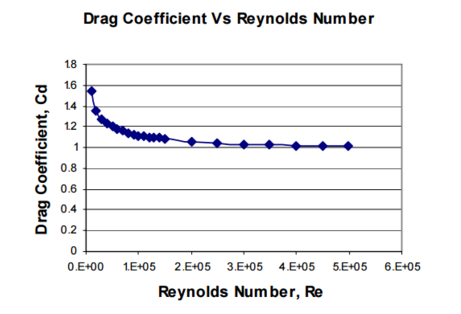
\includegraphics[width=0.9\textwidth]{figures/graphic-reynolds.png}
  \caption{Coeficiente de arrasto em função do número de Reynolds \cite{eng2008}}
  \label{fig:graphic-reynolds}
\end{figure}
\FloatBarrier
\par
[APLICANDO A EQ 1.......]

\subsection{A Escolha da Bomba}
O modelo proposto será uma bomba do tipo Bilge, com as seguintes características:
\begin{itemize}
\item Peso: aproximadamente 3 kg
\item Modelo: 1100 GPH - com Tensão de trabalho 12 V DC - Amperagem de 3,3;
\item Formato: Cilíndrico alterável;
\item Área de operação entorno de até 3,7 metros;
\end{itemize}

A bomba comercial a ser utilizada esta apresentada abaixo: 
\par
\begin{figure}[h]
  \centering
  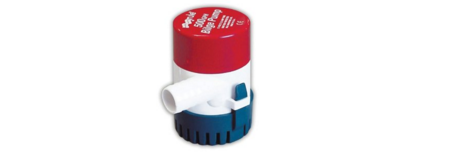
\includegraphics[width=0.9\textwidth]{figures/waterbomb.png}
  \caption{Bilge Pump}
  \label{fig:waterbomb}
\end{figure}
\FloatBarrier
\par

\section{A Fonte de Alimentação}
\subsection{O Dimensionamento}
A alimentação do Pool Clean Robot o cabo de energia foi dimensionado de forma a suprir a potência elétrica dos equipamentos embarcados no sistema além de garantir que o robô percorra, sem limitação de distância, toda a extensão da piscina. O Clean Pool Robot será alimentado por uma tomada perto da piscina, em tensão de 220V (padrão Brasília), entretanto os diversos equipamentos intermos são alimentados em diferentes tensões, fazendo com que seja necessário o uso de uma fonte chaveada para a redução da tensão de alimentação de cada equipamento.

O comprimento do cabo será explicado a seguir. Para o correto dimensionamento de um cabo de energia, de acordo com a literatura, deve-se levar em consideração a distância entre a fonte de energia e a carga, a potência consumida, além da queda de potência do cabo. Assim, o cálculo para a definição da bitola do fio que será utilizado fica determinado pela equação abaixo.

\begin{displaymath}
  S = \frac{\sqrt{3} \times IL}{58 \times U}
\end{displaymath}
Para um fio trifásico de cobre a equação apresenta o cálculo para o seu dimensionamento. Na equação S é a bitola do fio, em mm2, I é a corrente que passa pelo condutor, em Ampères, L é o comprimento total da fonte de energia até a carga, em metros, U é a queda de tensão suportada pelo fio, em Volts, e 58 é uma constante devido ao material do fio, no caso Cobre. Para o robô de piscina deste projeto a potência total consumida no robô é de 240W, assim a corrente que deverá ser suportada no fio é de 1,60 A. Assim, utilizando a equação acima temos que a bitola ideal para o fio será de 6,5 mm2, para o sistema ca.

A alimentação dos dois motores das escovas será feito com alimentação em cc, assim a figura abaixo apresenta modelo para cálculo da espessura do fio. Para o caso do robô, o fio de alimentação dos motores deverá suportar 1,5 mm2.
\par
\begin{figure}[h]
  \centering
  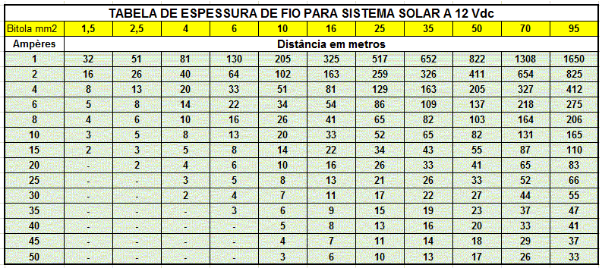
\includegraphics[width=0.9\textwidth]{figures/table-wire.png}
  \caption{Espessura de fio para sistemas solar 12 V em dc.}
  \label{fig:table-wire}
\end{figure}
\FloatBarrier
\par
Como a alimentação interna do robô deve ser feita em duas tensões diferentes, foi escolhido uma fonte chaveada (Switched-mode power supply, na língua inglesa). Essa fonte de alimentação elêtronica que incorpora um regulador chaveado, em outras palavras um circuito controlador interno que chaveia a corrente, ligando e desligando de forma rápida, mantendo, assim, uma tensão de saída estabilizada. Os parâmetros que serão suficientes para a alimentação do sistema estão explicados a seguir.

Ao contrário das fontes lineares, esse tipo de fonte se utiliza de circuitos embutidos fazendo com que este tipo de equipamento seja menor e mais leve, o que seria importante para o produto final, pois traria maior conforto ao cliente. Apresenta uma potência dissipada maior, pois utiliza de transistores do tipo FET( Filed Effect Transistor), dessa forma sendo mais vantajoso. Além de dissipar menor quantidade de calor por não apresentar um núcleo de ferro. Esses fatores fazem com que a eficiência desse tipo de equipamento seja melhor.

\subsection{Fonte Chaveada}
Devido a características de baixo volume e peso em comparação a fontes de alimentação convencionais, a fonte de alimentação chaveada é atualmente a mais utilizada em sistemas eletrônico. Importante evidenciar que as fontes chaveadas são sistemas eletrônicos bem mais complexos que as fontes de alimentação convencionais, visto que sua principal vantagem está relacionada à utilização de um interruptor eletrônico durante seu funcionamento [8].

Desse modo a potência elétrica pode ser definida de acordo com a tensão e corrente, sendo essa:
\begin{displaymath}
  P = V \times I
\end{displaymath}

Onde, $P$ é potência em Watts; $V$ é tensão em Volts e $I$ é a corrente em Ampére.

Com isso, quando um transistor está trabalhando na região linear como um controlador de corrente, a potência elétrica do sistema não será nulo gerando assim uma dissipação da potencia em forma de calor. Porém, se o transistor estiver operando como um interruptor, a mesma irá gerar uma dissipação de potência bem menor se comparada as demais fontes de alimentação, devido ao processo de chaveamento acontecer em intervalos pequenos [8].

Passando para parâmetros de eficiência, a fonte de alimentação com chaveamento apresenta uma relação de quase 95\% de qualidade em comparação as demais fontes de alimentação sem chaveamento, os quais ficam entorno de 65\%. Além da análise da relação de potência por peso, sendo às fontes convencionais capazes de fornecer 25W/kg e as fontes chaveadas capazes de oferecer 100W/kg [8].

Com base nas informações apresentadas e na possível potência geral do sistema está em torno de 240 Watts, serão utilizadas duas fontes de alimentação chaveada com os seguintes parâmetros elétricos : 110/220 Volts AC para 12 Volts e 10 Ampéres DC. Importante ressaltar que o sistema será alimentado por duas fontes independentes ao mesmo tempo, a fim de se evitar possíveis danos ao sistema eletrônico devido a corrente de partida dos motores de escovação e da bomba de propulsão.
\par
\begin{figure}[h]
  \centering
  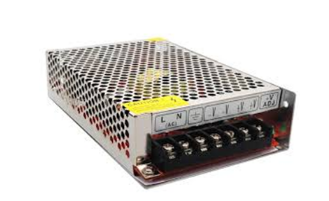
\includegraphics[width=0.6\textwidth]{figures/power-supply.png}
  \caption{Fonte de alimentação Chaveada. }
  \label{fig:power-supply}
\end{figure}
\FloatBarrier
\par

\section{Vedação}
O Clean Pool Robot possui diversos equipamentos eletrônicos em seu interior que não podem ter contato com água, portanto para o sistema de vedação realizou-se um estudo dos produtos presentes no mercado que podem realizar a vedação de objetos em água. A seguir apresentamos um breve descritivo dos principais. 

\begin{table}[]
\centering
\caption{My caption}
\label{my-label}
\begin{tabular}{|c|l|}
\hline
\begin{tabular}[c]{@{}c@{}}Cola\\ de\\ resorcinol\end{tabular}                   & \begin{tabular}[c]{@{}l@{}}É um adesivo à prova d'água e forma\\ ligas fortes e duráveis após sua cura,\\ mas a água a remove antes desta cura.\\ O tempo de cura é de 8 a 24 horas,\\ dependendo da umidade e temperatura.\\ A cola de resorcinol precisa de juntas justas,\\ sem folgas,e pressão forte para curar,\\ geralmente, essa pressão é aplicada\\ através de grandes presilhas em C ou presilhas\\ para cola.. (4) A cola de resorcinol tem\\ excelente resistência\\ às temperaturas extremas, produtos\\ químicos e fungos. (2)\end{tabular} \\ \hline
\begin{tabular}[c]{@{}c@{}}Cola\\ a base\\ de vinil\end{tabular}                 & \begin{tabular}[c]{@{}l@{}}O adesivo a base de vinil têm uma colagem\\ forte à prova d'água em vinil e em\\ muitos plásticos, mas não devem ser usadas\\ em espumas. Normalmente não é necessário\\ usar grampos. A cola de vinil\\ permanece clara e flexível; o tempo de\\ cura é de 10 a 20 min.(2)\end{tabular}                                                                                                                                                                                                                                        \\ \hline
\begin{tabular}[c]{@{}c@{}}Cola\\ a base\\ de epóxi\end{tabular}                 & \begin{tabular}[c]{@{}l@{}}As colas a base de epóxi são de duas\\ partes: uma resina é misturada a\\ um endurecedor, e ela cura por ação química, e\\ não ao ar, como os outros tipos.\\ Ela é a prova d'água, e é muito usada na\\ fabricação de barcos modernos em madeira. Não requer\\ juntas justas, mas preenche as folgas. \\ Precisa apenas de pressão moderada durante a fase de cura.(4)\end{tabular}                                                                                                                                            \\ \hline
\begin{tabular}[c]{@{}c@{}}Cola\\ a base\\ de poliuretano\end{tabular}           & \begin{tabular}[c]{@{}l@{}}As colas a base de poliuretano são aplicadas\\ diretamente do seu tubo, sem precisar de um endurecedor.\\ Ela requer uma junta justa, e\\ a aplicação de pressão durante o tempo de cura. A\\ "DIY Wood Boat" nota que\\ é preciso usar a umidade para curá-la corretamente,\\ então a madeira deve ser\\ levemente umedecida antes da aplicação da\\ cola nas superfícies que\\ ela unirá. Essas colas são a prova d'água. (4)\end{tabular}                                                                                    \\ \hline
\begin{tabular}[c]{@{}c@{}}Cola\\ a base\\ de ureia e\\ formaldeído\end{tabular} & \begin{tabular}[c]{@{}l@{}}A cola a base de ureia e formaldeído é uma\\ cola de três partes. Um pó deve ser misturado com\\ água para formar uma pasta. Depois,\\ um ácido é adicionado para iniciar o processo\\ de cura. É preciso ter juntas justas e alta pressão\\ para que sua adesão seja apropriada.\\ Ela é resistente à água, mas não completamente\\ a prova d'água.(4)\end{tabular}                                                                                                                                                            \\ \hline
\end{tabular}
\end{table}

Dos adesivos acima descritos, todos possuem uma grande desvantagem, são tóxicos e nem todos são completamente a prova d’água. Com base nisso, procurou-se outro produto no mercado. O Persilox se apresentou como um produto sustentável, não possui cheiro forte e não causa danos à saúde e nem ao meio ambiente, pois sua fórmula inovadora não contém solventes, isocianatos e nem ácidos. (3). Esse adesivo foi desenvolvido pela Universidade de São Paulo, em sua incubadora, possui um processo de cura é rápido, não retrai, e depois de curado, adquire alto poder de adesão e coesão. Fica completamente elástico, flexível, não trinca, apresentando alta performance em propriedades mecânicas, é resistente a intempéries, radiação UV e pode ser pintado com tintas a base d'água ou outros sistemas(1).

\subsection{O Persilox®}
O  Pesilox® é o adesivo a prova d’água, de alta resistênciao, que fará a vedação dos equipamentos elétricos internos.
\par
\begin{figure}[h]
  \centering
  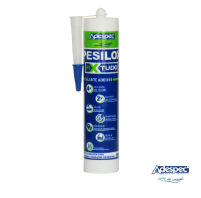
\includegraphics[width=0.2\textwidth]{figures/persilox.png}
  \caption{Adesivo Persilox®}
  \label{fig:persilox}
\end{figure}
\FloatBarrier
\par
O adesivo Persilox® é composto de uma mistura química não é tóxica, como os outros similares da categoria, pois é livre de tolueno, acetado de etila, dentre outros. O Persilox® é um adesivo, impermeabilizante e selante de alta performance que pode ser aplicado em todos os materiais, inclusive em pisos sujeitos a lavagem. O adesivo se solidifica ao entrar em contato com a umidade do ar e, por sua ausência de produtos tóxicos, pode ser aplicado com pano, mão ou pincel. A tabela abaixo apresenta as características do Persilox®.

\begin{table}[]
\centering
\caption{My caption}
\label{my-label}
\begin{tabular}{@{}|c|c|@{}}
\toprule
Propriedade                           & PERSILOX                  \\ \midrule
Base química                          & Pesilox                   \\ \midrule
Cor                                   & Preto/Cinza/Branco/Natura \\ \midrule
Mecanismo de Cura                     & Umidade                   \\ \midrule
Densidade                             & 1,35 - 1,40 g/cm\textsuperscript{3}         \\ \midrule
Estabilidade                          & Boa                       \\ \midrule
Temperatura de aplicação              & ambiente                  \\ \midrule
temperatura de formação de película   & 10 minutos                \\ \midrule
Tempo de trabalho                     & 10 minutos                \\ \midrule
Resistência a tração                  & 18 Kgf/cm\textsuperscript{2}                \\ \midrule
Tempo de armazenagem (abaixo de 25ºC) & 12 meses                  \\ \midrule
Resistência a Temperatura             & -40ºC a 120ºC             \\ \midrule
Resistência química                   & muito boa                 \\ \midrule
Trincamento                           & nenhum                    \\ \bottomrule
\end{tabular}
\end{table}

O Persilox® foi utilizado pelo grupo para fazer a vedação da parte elétrica interno do robo. Para testar a eficácia do produto foi feito um teste.

\section{A Mente do Robô (Eletrônica e Software)}
\par
\begin{figure}[h]
  \centering
  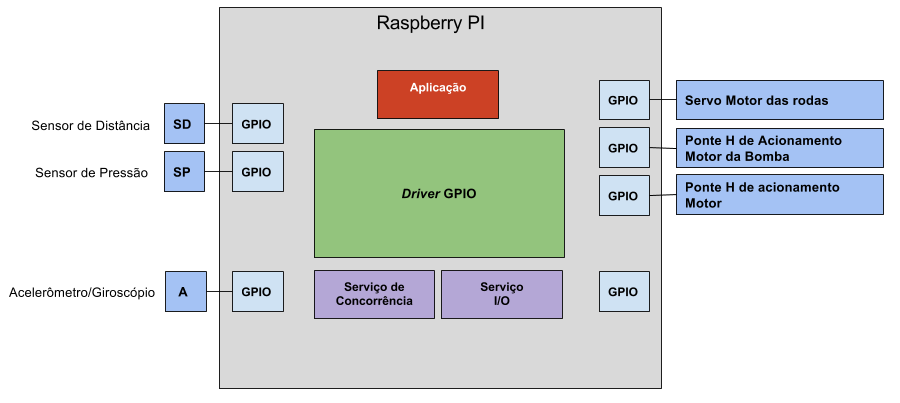
\includegraphics[width=0.8\textwidth]{figures/schema-eletro-soft.png}
  \caption{Interação dos componentes eletrônicos e o core software.}
  \label{fig:schema-eletro-soft}
\end{figure}
\FloatBarrier
\par
Os periféricos fornecerão dados que, por sua vez, serão passados ao driver por meio de dispositivo de hardware (GPIO).  O driver será responsável por permitir a comunicação entre o hardware e o software que, na figura, é representado pelos serviços que deve fornecer ao sistema. Cada serviço tratará os dados de entrada conforme a especificidade solicitada e, em seguida, retorna uma saída para um atuador, por meio do driver.

\subsection{Central de Processamentos de Dados}
\subsubsection{Os Requisitos}
Na seleção de uma unidade de processamento o maior fator de seleção foi conseguir uma de forma rápida e com baixo custo, além de ter uma capacidade de processamento suficiente para solucionar os primeiros requisitos vistos da integração entre a área Estrutural (sensores necessários para funcionamento e acionamento de motores e bombas) e a área de software (capacidade de programar em várias linguagens de programação e uso de APIs), e ter acesso a GPIO. Considerando esses fatos a primeira proposta foi a Raspberry pi, porém por sua limitação de pinos GPIO e a necessidade de muitos pinos para analisar sinais analógicos, foi proposto usar também um arduino, que vem com conversor A/D e já estava disponível para uso. Isso proporcionou a continuidade do trabalho de implementação que já vinha sendo feito sem muitas mudanças devido a alterações trazidas pela área eletrônica.
\par
\begin{figure}[h]
  \centering
  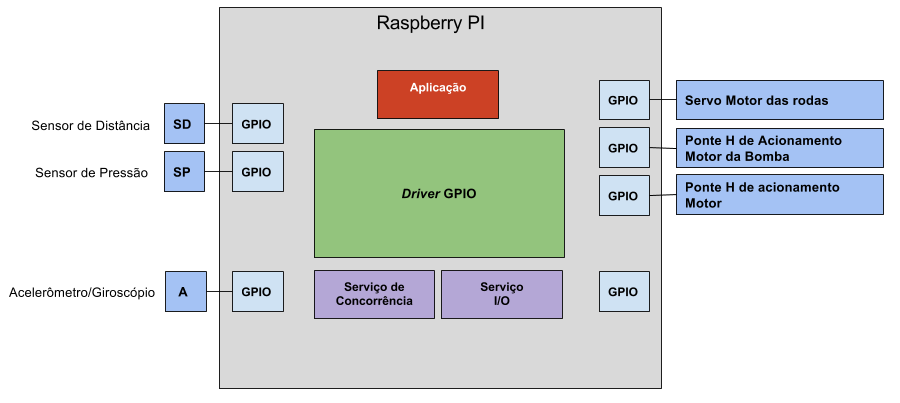
\includegraphics[width=0.8\textwidth]{figures/schema-eletro-soft.png}
  \caption{Interação dos componentes eletrônicos e o core software.}
  \label{fig:schema-eletro-soft}
\end{figure}
\FloatBarrier
\par

\subsubsection{Raspberry PI 2 B}
Com o objetivo de desenvolver um robô é necessário ter uma central de processamento de dados. A Raspberry pi foi escolhida pela sua capacidade de processamento onde pode ser processado as variáveis que fazem o robô tomar decisões na sua rotina. A Raspberry aciona a passagem de energia em  relés que fazem o acionamento dos motores que giram as escovas, e do motor da bomba. Como a Raspberry não tem conversor A/D foi necesário usar um arduino para tratar o sensor de pressão. A comunicação da Raspberry com o Arduino é feito usando protocolo serial  UART (Universal Asynchronous Receiver/Transmitter). Também há a possibilidade do uso de várias linguagens de programação e APIs.
\par
\begin{figure}[h]
  \centering
  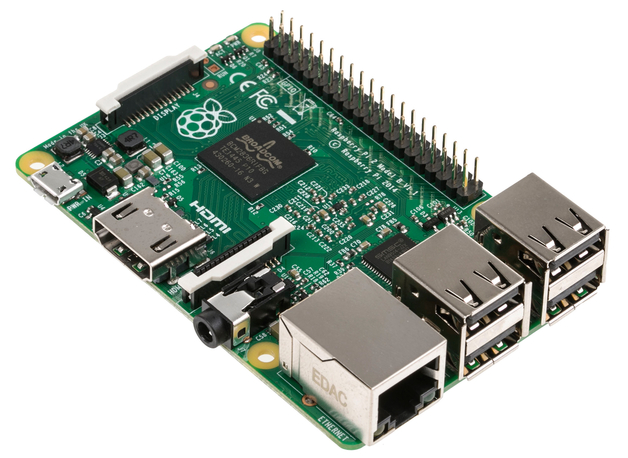
\includegraphics[width=0.8\textwidth]{figures/rpi2b.jpg}
  \caption{Raspberry PI 2 B.}
  \label{fig:schema-eletro-soft}
\end{figure}
\FloatBarrier
\par

\subsubsection{Arduino}
O Arduino Uno foi escolhido a princípio para facilitar o tratamento do sensor de pressão MPX-4250, que possui saída analógica. Trabalhar com   conversão A/D na raspberry pi requer o uso demasiado de pinos ( no mínimo 9 pinos para controlar dois sensores, utilizando-se de multiplexadores. ).  Uma vez que o Arduino Uno foi incluido no sistema, delegou-se  a ele também o trabalho de controlar os sensores de distancia HC-SR04, visto  que  estes são modulos desenvolvidos para funcionar no arduino.
\par
\begin{figure}[h]
  \centering
  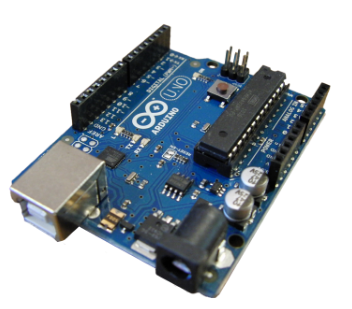
\includegraphics[width=0.8\textwidth]{figures/arduino.png}
  \caption{Arduino.}
  \label{fig:arduino}
\end{figure}
\FloatBarrier
\par

\subsection{O Sistema de Controle de Tensão}
\subsubsection{Os Requisistos/Dimensionamento}
Para acionar os sistemas de alta tensão (Motores e Bomba) com circuitos de baixa tensão (Raspberry) foram utilizados relés. Com baixas tensões ele induz um campo eletromagnético sobre uma bobina, o que faz com que o relé deixe passar a tensão que está normalmente fechado, caso não haja essa alimentação o relé mantém-se emaberto, efetivamente funcionando como um interruptor.  Como é desejado que em um dos estados o circuito acione o motor e no outro o motor não funcione, foi projetado o circuito electrônico para só acionar o motor em normalmente fechado, em normalmente aberto o motor está em circuito aberto não sendo acionado.
\par
\begin{figure}[h]
  \centering
  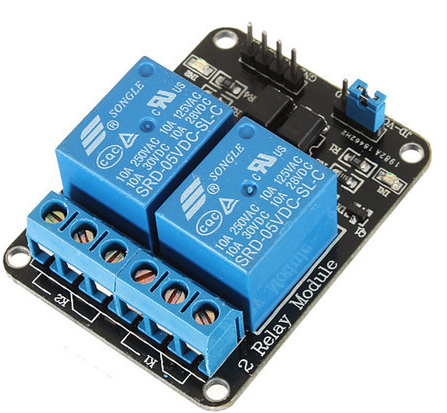
\includegraphics[width=0.8\textwidth]{figures/rele.png}
  \caption{Rele de dois modulos modelo SRD-05VDC-SL-C.}
  \label{fig:rele}
\end{figure}
\FloatBarrier
\par

\subsubsection{GPIO - \textit{Generic Ports Input/Output}}
Generic Ports Input Output são saídas e entradas de tensão. Elas servem para fazer a comunicação do processador com componentes externos, sensores e atuadores e outros tipos de componentes eletrônicos. Algumas dessas portas tem usos predefinidos pelo fabricante do Hardware como saídas de alimentação genérica, e terras, outras dos pinos são de uso genérico. A Raspberry Pi tem 40 GPIO, das quais  17 são para uso genérico.
\par
\begin{figure}[h]
  \centering
  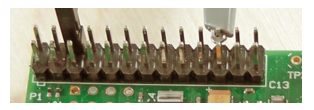
\includegraphics[width=0.8\textwidth]{figures/gpio.png}
  \caption{GPIO Raspberry 1.}
  \label{fig:gpio}
\end{figure}
\FloatBarrier
\par

\subsubsection{\textit{Driver} GPIO}
O driver GPIO é um software que habilita a comunicação entre o hardware e o software. A partir do driver é possível receber  os dados advindos dos componentes de hardware, fazer o devido tratamento e, se necessário, enviar uma resposta ao hardware (WINDOWS). Para o projeto foram identificadas algumas bibliotecas, disponibilizadas pela comunidade que utiliza o Raspberry. Essas bibliotecas fazem a interface entre o hardware e o middleware, de forma que essas APIs fazem o papel do driver.

\subsection{O Sistema de Sensoriamento}
\subsubsection{Os Requisitos/Dimensionamento}
Para garantir que o robô seja capaz de seguir o percurso definido é necessário que ele seja capaz de detectar as quatro paredes conforme se aproxima de alguma delas. Para tanto, quatro sensores de distância devem ser posicionados em cada uma das laterais do robô. Em caso de colisão com algum obstáculo não detectado pelos sensores de distância e a fim de manter constante o movimento em linha reta do robô, um acelerômetro/giroscópio deve ser utilizado no sistema. Por fim, tanto a pressão interna da caixa de filtragem quanto a externa do robô devem ser medidas constantemente. Caso haja o bloqueio da sucção da bomba por algum detrito haverá também uma variação da pressão interna, que pode ser detectada pelo sensor de pressão e permitir uma resposta imediata do sistema. Para garantir que o robô encontra-se de fato no fundo da piscina conforme ele segue seu percurso, a pressão externa do robô deve ser medida também.

\subsubsection{Os Sensores}
\begin{description}
\item[Sensores de Distância:] serão utilizados sensores de distância com o intuito de permitir ao robô a identificação do espaço entre o robô e qualquer objeto à sua frente. Isso é importante para evitar colisões com as paredes da piscina e obstáculos a alturas que o sensor possa detectar. O sensor de distância ultrasônico HC-SR04 foi escolhido  por ser um módulo periférico próprio do arduino, facilitando assim sua implementação. Testes do sensor de baixo d'água ainda precisam ser realizados para validar a escolha.
\item[Sensor de Pressão:] O sensor de pressão proposto funciona com o princípios de materiais piezoelétricos, um liquido entra dentro da câmara e proporciona uma pressão nas paredes da câmara, esse pressão gera uma diferença de potencial no material. Com essa diferença de potencial é possível, usando um conversor AD (Analógico/Digital), saber a pressão dentro da câmara. Esse sensor sera utilizado para medir a pressão dentro da câmara a onde se encontra a bomba de sucção, assim permitindo que a bomba só trabalhe dentro da pressão ideal de funcionamento, caso algo entupa a entrada da sucção esse sensor detectará  uma queda na pressão interna e por software o problema sera tratado.
\par
\begin{figure}[h]
  \centering
  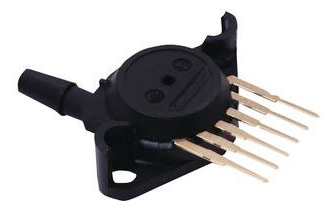
\includegraphics[width=0.4\textwidth]{figures/pressure-sensor.png}
  \caption{Sensor de Pressão}
  \label{fig:a}
\end{figure}
\FloatBarrier
\par
\item[Acelerômetro:] Está sendo cogitado usar um acelerômetro para auxiliar o deslocamento em linha reta do robô e detectar choques com obstáculos grandes, quando ocorre um choque com um obstaculo grande não detectado pelo sensor de distancia a uma variação brusca na aceleração, com isso podemos tratar o obstaculo ou abortar o funcionamento do robô.No mesmo modulo se encontra um giroscópio, ele mede rotações no robô, caso seja identificado alguma rotação não pretendida pelo sistema podemos usar esse dado para corrigir a trajetória do mesmo. O componente eletrônico que tem os dois sensores se comunica através do protocolo I2C. Isso reduz o numero de pinos necessários pare ler os dados do sensor.
\par
\begin{figure}[h]
  \centering
  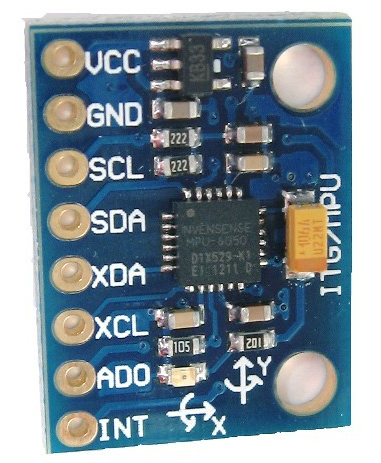
\includegraphics[width=0.4\textwidth]{figures/accelerometer.png}
  \caption{Acelerômetro}
  \label{fig:gpi}
\end{figure}
\FloatBarrier
\par
\end{description}

\subsection{O Sistema de Rotação do Robô}
\subsubsection{Os Requisitos/Dimensionamento}
Foi definido pelo projeto que a propulsão do robô será gerada pela bomba de filtragem. Neste contexto e considerando que o robô move-se idealmente apenas em quatro direcões, existiam duas opções de controle da saída de água da bomba para o controle do direcionamento. A primeira, mais simples, consistia em dispor quatro canos de saída no topo do robô e, por meio de válvulas, controlar quais das saídas seriam abertas de cada vez. A segunda, mais elaborada, consiste em dispor um único cano capaz de rotacionar em 360 graus para se posicionar na direção desejada conforme o robô segue seu percurso. Foi decidido que a segunda opção seria a melhor alternativa, pois ela permite, juntamente com o acelerômetro/giroscópio, corrigir em tempo real qualquer desvio significativo da rota que o robô possa vir a sofrer.

	Conforme o robô segue seu percurso, as rodas devem ser capazes de se manter em duas posicões: horizontal e vertical. Para tanto, um sistema de servos com rotação de 180 graus foi escolhido, similar ao esquema de propulsão.

\subsubsection{Servo Motor}
Servos motores são utilizados para rotacionar um eixo até uma posição desejada. Esses motores são normalmente motores de alto torque. Dois servos (Micro Servo 9g SG90 TowerPro) serão utilizados para rotacionar as rodas (5), o principal motivo de escolher esse modelo é ele ter torque suficiente para mover as mesmas e ter baixo custo, E para mover a saída de água (4) da bomba foi escolhido um servo motor (SM-S4306R) com maior liberdade de rotação (360º) e uma maior torque.
\begin{figure}[h]
  \centering
	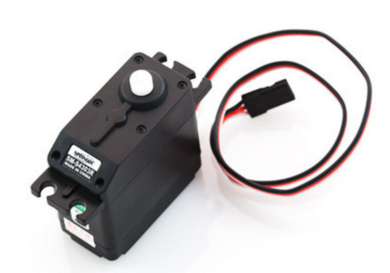
\includegraphics[height=5cm]{figures/servant-motor.png}
	\quad
	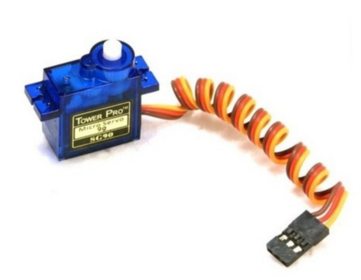
\includegraphics[height=5cm]{figures/micro-motor.png}
  \caption{Servo Motores \cite{flipflop2013} e \cite{flipflop2016}, respectivamente}
\end{figure}
\FloatBarrier

\subsection{Circuito Desenvolvido}
\subsubsection{Diagrama do Circuito}
A figura abaixo mostra o diagrama do circuito proposto:
\par
\begin{figure}[h]
  \centering
  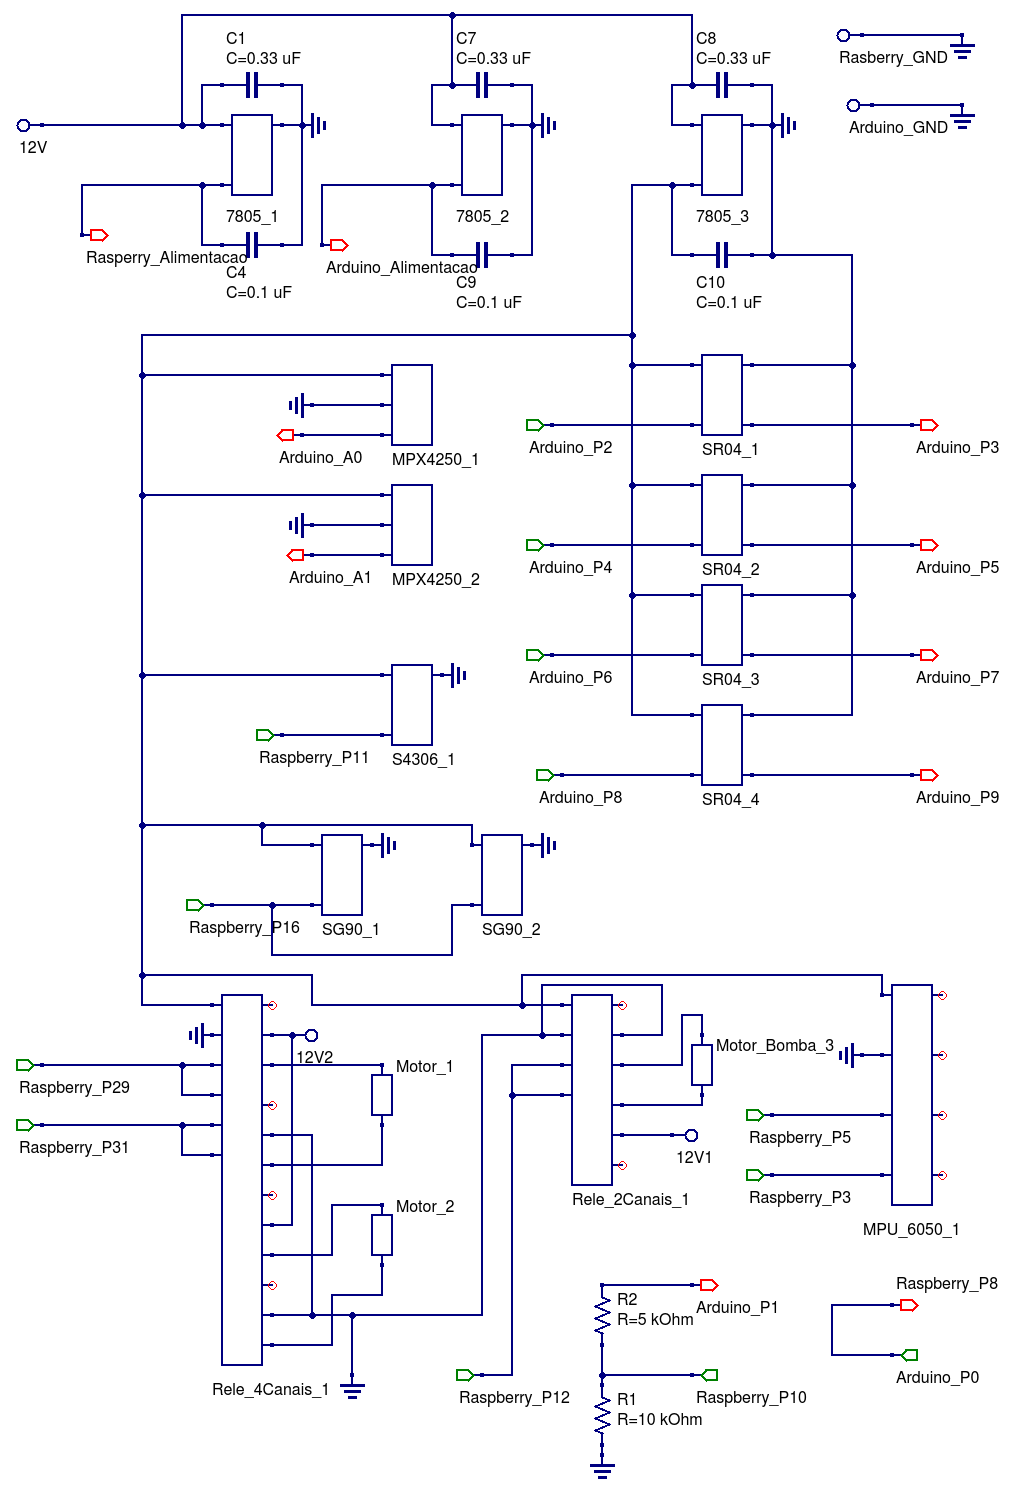
\includegraphics[width=0.8\textwidth]{figures/circuit.png}
  \caption{Circuito proposto.}
  \label{fig:circuit}
\end{figure}
\FloatBarrier
\par

Para a alimentação da raspberry Pi 2 e do Arduino Uno, bem como todos os componentes alimentados em 5V (servo motores, sensores de distância, sensores de pressão), a partir dos 12V oferecidos pela fonte, utilizaram-se reguladores de tensão 7805. Capacitores de 0.33 e 0.1uF foram colocados em paralelo aos reguladores de tensão como medida de segurança.

Conectados a raspberry Pi 2 estão os servo motores SG90 e e S4306, pelos pinos 16 e 11 respectivamente. Para o controle dos motores das escovas e da bomba, utilizaram-se relés para fazer o chaveamento com a tensão de 12V da fonte. O acelerômetro/giroscópio MPU\_6050 é conectado a Pi via Barramento Serial I2C , para conectar periféricos de baixa velocidade a um sistema embarcado.

A raspberry Pi 2 e o Arduino Uno são conectados por porta serial TX e RX e se comunicam via UART (Universal Asynchronous Receiver/Transmitter). Um divisor de tensão é usado para conectar o pino TX0 de 5V do Arduino ao pino RXD de 3.3V da Raspberry Pi2.

No Arduino estão conectados os quatro sensores de distância SR04 em portas digitais e os dois sensores de pressão MPX4250 nas portas analógicas A0 e A1.

Até o momento da produção deste relatório, todos os componentes do circuito acima foram testados individualmente, a excessão do acelerômetro e dos relés (ainda a serem obtidos). A montagem do circuito completo em PCB ou placa universal ainda não foi iniciada.

\subsubsection{Pinagem}
A Figura abaixo mostra a pinagem de cada componente eletrônico do circuito.
\par
\begin{figure}[h]
  \centering
  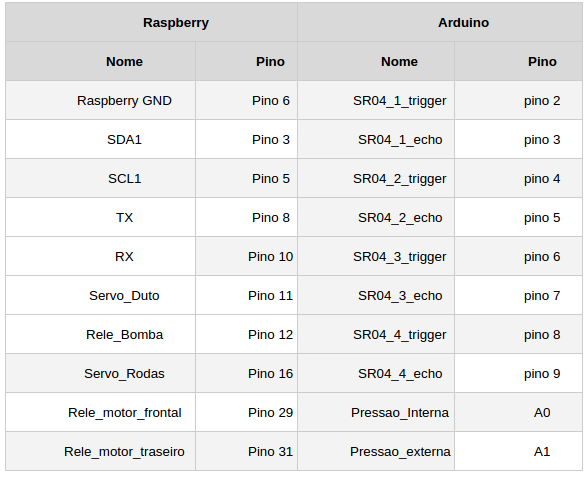
\includegraphics[width=0.8\textwidth]{figures/pinout.png}
  \caption{Pinagem usada.}
  \label{fig:pinout}
\end{figure}
\FloatBarrier
\par

\subsection{Programação e Arquitetura de Software}
A linguagem de programação selecionada inicialmente foi C++ e a biblioteca BCM2835.h para servir como driver de comunicação entre o software e o hardware. No entanto, houve a incompatibilidade entre essa biblioteca e a Raspberry pi 2. A documentação dessa biblioteca (McCauley) diz que ela foi desenhada para funcionar na versão 1 da Raspberry, mas era compatível com a versão 2, desde que tomadas algumas providências de configuração. Após ter-se feito todo o necessário ainda não estava funcionando corretamente, de forma que a equipe tomou a decisão de mudar de linguagem para Python 2.7, que também possui uma biblioteca de comunicação com a GPIO.

A escolha pela BCM2835.h e C++ foram escolhas em que já se sabia dos riscos e que já foram contornados. Tomada a decisão todo o trabalho já foi convertido para a nova linguagem e vem se mostrando funcional.

A figura abaixo mostra a abstração da arquitetura do sistema associado ao projeto.
\par
\begin{figure}[h]
  \centering
  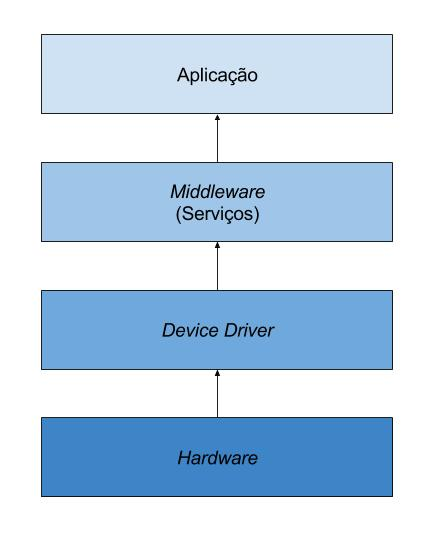
\includegraphics[width=0.4\textwidth]{figures/schema-arch.jpg}
  \caption{Visão geral da arquitetura de software.}
  \label{fig:schema-arch}
\end{figure}
\FloatBarrier
\par

\subsubsection{\textit{Middleware}}
Middleware é um software que conecta outros componentes de software. Uma camada de infraestrutura que viabiliza o desenvolvimento de aplicações voltadas ao negócio. Provê serviços que serão amplamente utilizados pela aplicação de negócio (ORACLE). O middleware fornecerá serviços base para o robô, como ativação dos motores, escova e uso dos sensores.

\subsubsection{Camada de Serviços}
\subsubsubsection{Os Requisitos}
Por meio de reuniões com a equipe de Estruturas a equipe de Lógica identificou algumas ações que o robô precisaria fazer:
\begin{itemize}
\item Identificação de profundidade na piscina.
\item Constante análise da distância entre o robô e obstâculos.
\item Acionamento dos diversos sistemas do robô, como locomoção e filtragem.
\item Comunicação entre os dois componentes do sistema de processamento de dados.
\end{itemize}

A partir desse levantamento e considerando como comumente é definida arquitetura para softwares em sistemas embarcados, percebeu-se a necessidade de dois serviços: um serviço para comunicação (entrada/saída de dados) e um para lidar com concorrência de requisições. Assim, a Figura abaixo detalha melhor a comunicação entre as camadas propostas da arquitetura, considerando-se os serviços a serem utilizados e as funcionalidades na camada da aplicação.

\par
\begin{figure}[h]
  \centering
  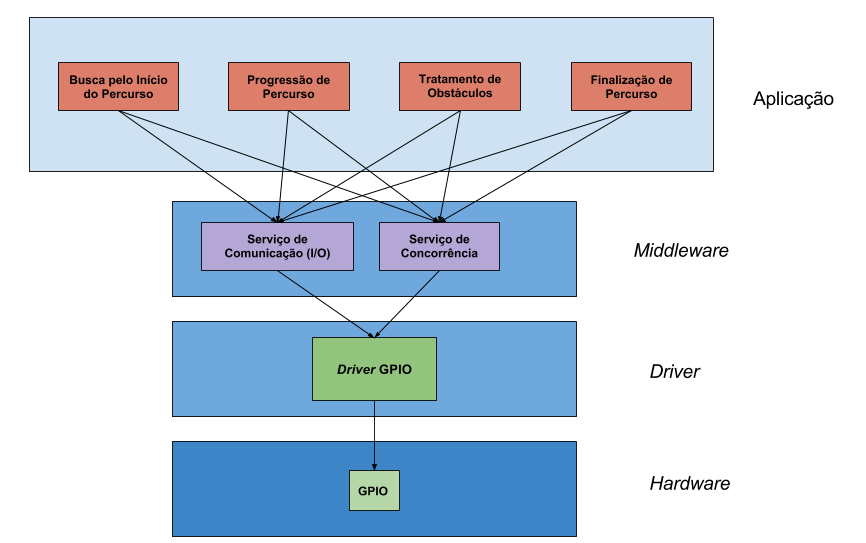
\includegraphics[width=0.8\textwidth]{figures/layers-soft.png}
  \caption{Visão detalhada das camadas de software.}
  \label{fig:layer-soft}
\end{figure}
\FloatBarrier
\par

\subsubsubsection{Serviço de Comunicação (I/O)}
Esse serviço tem por propósito fazer a ponte de comunicação entre o driver e a aplicação. Dessa forma, a camada de serviço, por meio do serviço de I/O, deixa invisível para a camada de aplicação como se dá o processo de comunicação com as camadas mais baixas. Isso permite melhor entendimento do código, bem como a possibilidade de refatoração mais simples, na medida em que há um desacoplamento entre as duas partes, comunicação e aplicação. Assim, uma alteração na camada de serviço não terá impacto na camada superior, de serviço, pois a interface entre as duas se manterá. As mudanças internas à camada não interferem no funcionamento de outra.

Abaixo segue a listagem do código até o momento do serviço de comunicação.
\begin{lstlisting}[language=Python, label=services, caption=Código da Camada de Serviços]
import pinout as pin
import time
import serial
import RPi.GPIO as GPIO
import time 
#Configura a serial e a velocidade de transmissao
#pmw=GPIO.PWM(pinout.SERVO_WHEELS,50)
#pmw.start(5)

mw_dute = GPIO.PWM(pin.SERVO_PUMP,50)
pmw_dute.start(5) 
def start_arduino():
    arduino_communication = serial.Serial("/dev/ttyAMA0", 115200)
    return arduino_communication

def read_arduino(arduino_communication):
    response = arduino_communication.readline()
    return response     

def write_arduino(arduino_communication, line):
    arduino_communication.write(line)
    return

def activate_pump():
   GPIO.output(pin.WATER_PUMP, GPIO.HIGH)
    return True

def deactive_pump():
    GPIO.output(pin.WATER_PUMP, GPIO.LOW)
    return False

def activate_brush():
    GPIO.output(pin.BRUSH, GPIO.HIGH)
    return True

def deactive_brush():
    GPIO.output(pin.BRUSH, GPIO.LOW)
    return False

def turn_servos_wheels(angle):
    duty = float(angle)/20 + 2.5
    pmw.ChangeDutyCycle(duty)      
    return

def turn_servo_pump(angle, direction):
    time_s = angle/270
    if (direction == 1):
        pmw_dute.ChangeDutyCycle(50)
        time.sleep(time_s)  
    else:
        pmw_dute.ChangeDutyCycle(2.5)   
        time.sleep(time_s)

    pmw_dute.ChangeDutyCycle(100) 
    return
\end{lstlisting}

\subsubsubsection{Serviço de Concorrência}
O serviço de concorrência tem por objetivo abstrair da aplicação questões relacionadas a tarefas que fazem uso do processamento ou de um canal ao mesmo tempo. Isso será comum nas tarefas relativas aos sensores, que devem estar aptos a exercerem suas funções o máximo de tempo possível. Assim, o serviço de concorrência fica responsável por permitir que eles atuem nesses termos, sem que um interfira nas atividades do outro.

\subsubsection{Camada de Aplicação}
A camada de aplicação da arquitetura fica responsável pelas ações mais alto nível, como locomoção e tomada de decisões. Ela solicita informações para a camada abaixo, a de serviços, e com esses dados faz o tratamento.

Foi escolhida a ação de percorrer o percurso para se trabalhar inicialmente, pois é a que traz mais valor de negócio ao cliente. O robô, após estar na posição inicial numa das quinas da piscina, inicia a sua caminhada até encontrar a próxima parede. Em seguida ele desloca-se para a direita aproximadamente 20 centímetros para então movimentar-se dando “ré”. Ao alcançar a parede faz o deslocamento novamente para a direita de 20 centímetros e repete o processo até encontrar a quina final.

Para essa tarefa o código faz uso dos serviços citados anteriormente e de um conjunto de tomadas de decisões baseadas nos dados recebidos dos serviços. Para demonstrar esse processo foi feito um diagrama de fluxo de dados, apresentado abaixo:
\par
\begin{figure}[h]
  \centering
  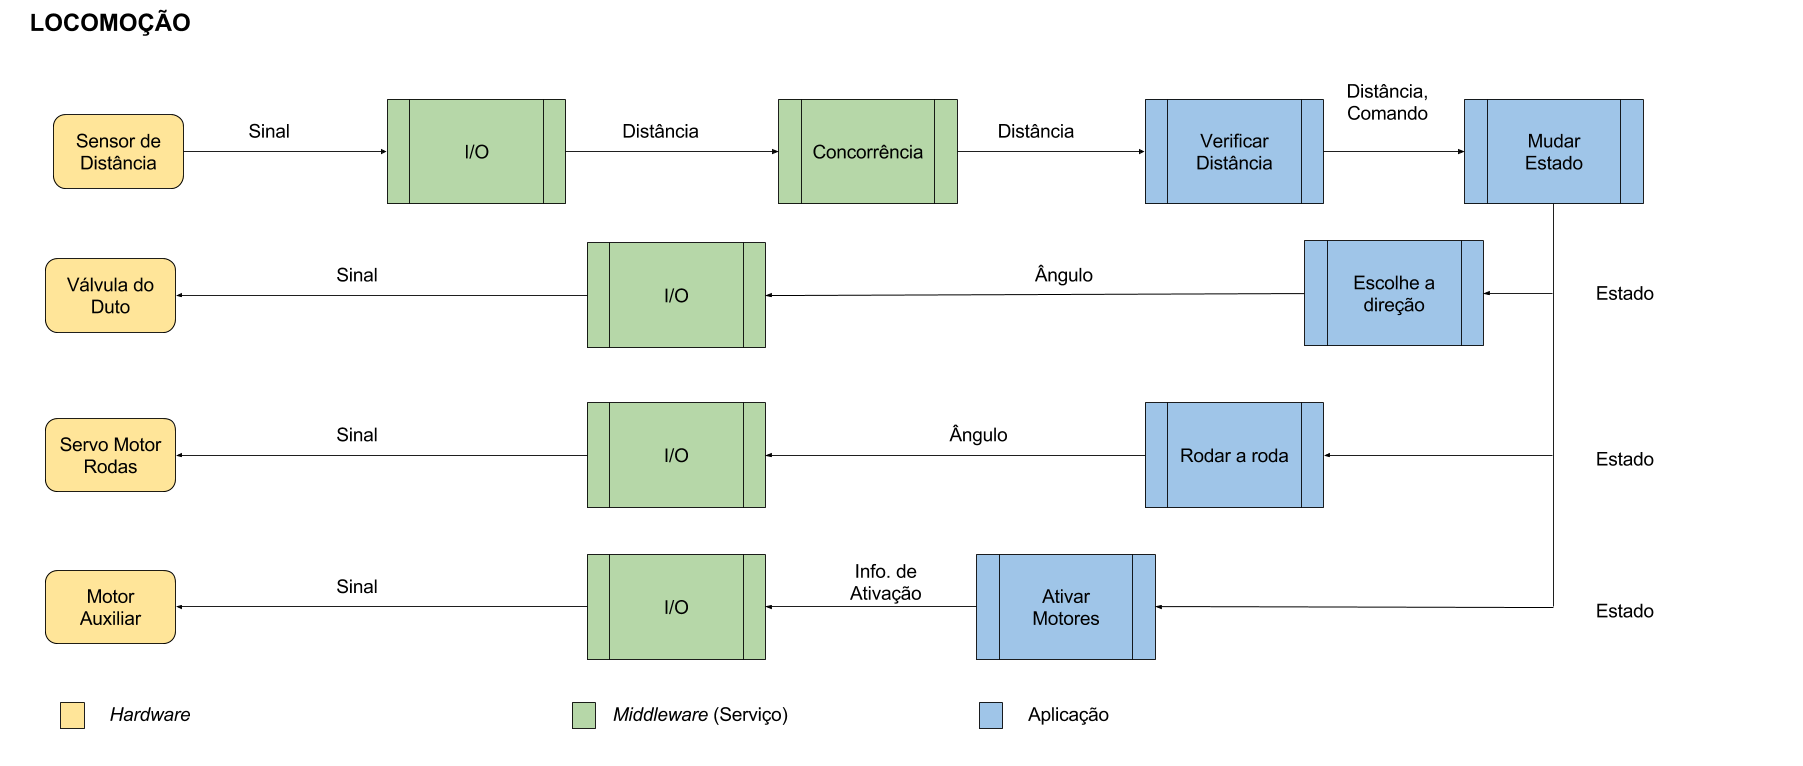
\includegraphics[width=0.8\textwidth]{figures/move-dfd.png}
  \caption{Diagrama de Fluxo de Dados para a Locomoção.}
  \label{fig:move-dfd}
\end{figure}
\FloatBarrier
\par
O código fonte é listado abaixo:

\begin{lstlisting}[language=Python, label=services, caption=Código da Camada de Aplicação]
import time
import communication as SERVICE


FOREVER = True
FRONT = 0
RIGHT = 90
BACK = 180
SIDEWAY = 90
VERTICAL = 0


def find_corner():
    # TODO: Think about the logic of how the CleanPoolRobot will find the
    #       corner of the pool.
    #
    return


def activate_water_pump():
    SERVICE.activate_pump()
    return


def deactivate_water_pump():
    SERVICE.deactive_pump()
    return


def turn_pipe(angle):
    return


def turn_wheels(angle):
    return


def read_front_distance_sensor():
    return 0


def read_back_distance_sensor():
    return 0


def read_right_distance_sensor():
    return 0


def read_left_distance_sensor():
    return 0


def deactivate_brush():
    return 0


def move_front():
    deactivate_water_pump()
    turn_pipe(FRONT)  # degree
    turn_wheels(VERTICAL)  # degree

    activate_water_pump()

    while FOREVER:
        distance = read_front_distance_sensor()  # cm

        if distance <= 5:
            deactivate_water_pump()
            deactivate_brush()
            break

    return


def move_right():
    five_seconds = 5

    deactivate_water_pump()
    turn_pipe(RIGHT)
    turn_wheels(SIDEWAY)

    activate_water_pump()
    time.sleep(five_seconds)  # second

    deactivate_water_pump

    return


def move_back():
    five_centimeters = 5

    deactivate_water_pump()
    turn_pipe(BACK)
    turn_wheels(VERTICAL)

    activate_water_pump()

    while FOREVER:
        distance = read_back_distance_sensor()  # cm

        if distance <= five_centimeters:
            deactivate_water_pump()
            deactivate_brush()
            break

    return


def state_machine(state):
    front = 1
    right = 2
    back = 3

    if state == front:
        move_front()

        previous_state = state
        state = right
    elif state == right:
        move_right()

        if previous_state == front:
            state = back
        else:
            state = front

    elif state == back:
        move_back()

        previous_state = state
        state = right

    return state


def route_course():
    activate_water_pump()

    state = 1

    while FOREVER:
        front_sensor = read_front_distance_sensor()
        back_sensor = read_back_distance_sensor()
        right_sensor = read_right_distance_sensor()
        left_sensor = read_left_distance_sensor()

        if (front_sensor > 5 and right_sensor > 5) or\
           (back_sensor > 5 and left_sensor > 5):
            break

        state = state_machine(state)

    return


def finish():
    # TODO: Think about the logic of how the CleanPoolRobot will turn back
    #       when it finish clean the pool.
    #
    return


def main():
    find_corner()
    route_course()
    finish()

    return

main()
\end{lstlisting}

\chapter{Montagem do Robô}
\section{Modelagem da Base do Robô}
Foi adquirida uma placa de aço de dimensões 500 mm de largura 900 mm de comprimento e 1,6 mm de espessura. Para se adequar ao projeto a placa foi reduzida para a seguinte dimensão 520 x 270 mm2 com a utilização de uma serra  tico-tico.

\par
\begin{figure}[h]
  \centering
  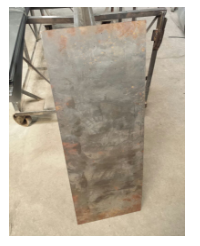
\includegraphics[width=0.4\textwidth]{figures/placa.png}
  \caption{Placa de aço adquirida.}
  \label{fig:placa}
\end{figure}
\FloatBarrier
\par

A serra “tico” e máquina esmerilhadeira foram usadas posteriormente para a realização dos cortes definidos para o contorno da placa e para realizar os dois furos referente as duas entradas de água, conforme as figuras. 

\par
\begin{figure}[h]
  \centering
  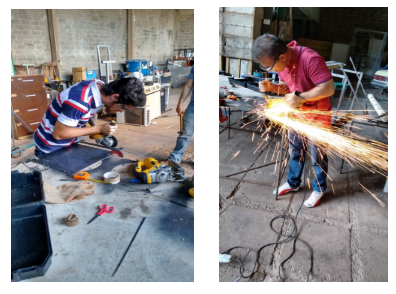
\includegraphics[width=0.5\textwidth]{figures/workers.png}
  \caption{Membros do grupo finalizando a modelagem da placa com a esmerilhadeira.}
  \label{fig:workers}
\end{figure}
\FloatBarrier
\par

Após as modificações a placa adquiriu as mesmas dimensões do sketch pré definido.

\par
\begin{figure}[h]
  \centering
  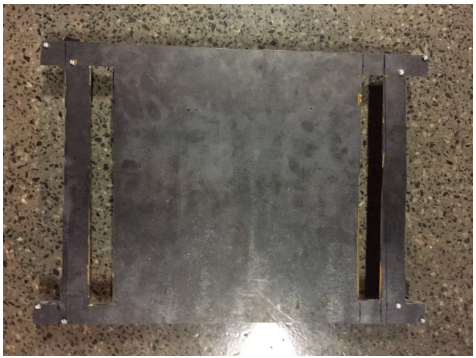
\includegraphics[width=0.4\textwidth]{figures/sketch-base.png}
  \caption{Sketch da base do robô.}
  \label{fig:sketch-base}
\end{figure}
\FloatBarrier
\par

\section{Construção dos Rolos de Limpeza}
Pela dificuldade de se encontrar as escovas, que irão realizar uma das partes da limpeza no processo do Clean Pool Robot, a equipe optou por utilizar uma feita pelos integrantes da equipe.

Foi utilizado um tubo cilíndrico de 300x50mm de PVC como base da estrutura dos rolos, e as “cerdas” das escovas foi  utilizado um polimero de fibra de vinil. Esse polimero foi cortado de maneira que seu comprimento fosse o mesmo comprimento da circuferência do tubo de PVC, afim de não existir nenhuma saliência que pudesse prejudicar a limpeza ou movimento do robô.
	
Para a fixação desse polímero no tubo foi utilizado um adesivo de contato tradicional da marca Cascola para se fazer a união desses dois materiais, depois disso o conjunto polímero e tubo, foi amarrado para que o adesivo estivesse seco e fosse bem aderido para que no momento de uso do robô o polímero não se desprendesse e por consequência não realizasse a escovação. O processo de produção pode ser acompanhado na Figura.

\par
\begin{figure}[h]
  \centering
  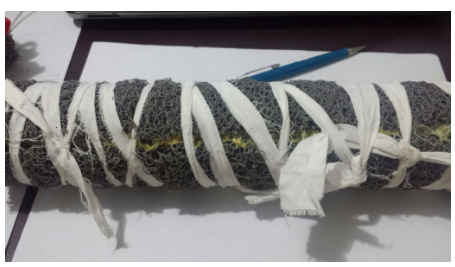
\includegraphics[width=0.4\textwidth]{figures/rolo.png}
  \caption{Processo de fabricação dos rolos de limpeza.}
  \label{fig:rolo}
\end{figure}
\FloatBarrier
\par

Foram confeccionadas duas escovas as quais resultaram na seguinte figura.

\par
\begin{figure}[h]
  \centering
  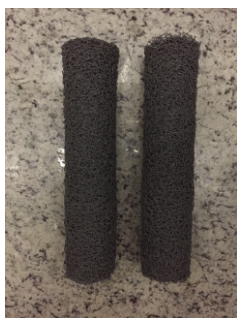
\includegraphics[width=0.5\textwidth]{figures/rolo-fim.png}
  \caption{Rolos de limpeza finalizadas.}
  \label{fig:rolo-fim}
\end{figure}
\FloatBarrier
\par

\section{instalação das Rodas}
Para realizar a instalação das quatro rodas, foi utilizado uma furadeira de bancada onde foram realizados furos para fixação das rodas. Foi utilizado uma broca número 5 e realizado o furo na placa de aço.

\par
\begin{figure}[h]
  \centering
  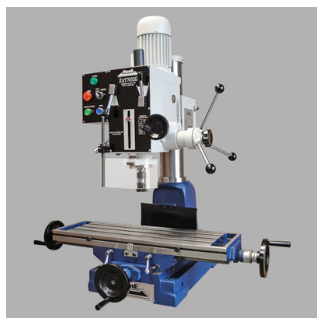
\includegraphics[width=0.4\textwidth]{figures/furadeira.png}
  \caption{Furadeira de bancada utilizada na fixação das rodinhas.}
  \label{fig:furadeira}
\end{figure}
\FloatBarrier
\par

Posteriormente foram fixadas as rodas na placa com parafusos e porcas.

\par
\begin{figure}[h]
  \centering
  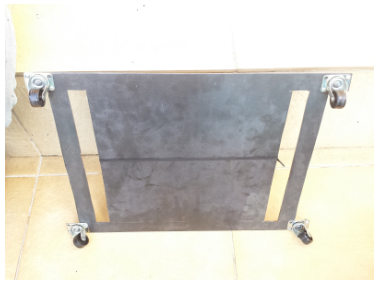
\includegraphics[width=0.6\textwidth]{figures/rodinhas.png}
  \caption{Rodinhas finalizadas na base.}
  \label{fig:rodinhas}
\end{figure}
\FloatBarrier
\par

\chapter{Testes do \textit{Clean Pool Robot}}
\section{Teste de Vedação - Persilox}
O teste do Persilox® teve por objetivo testar a eficácia do produto de vedação escolhido. Para tanto foi feito com o uso de um cabo, recipiente cilíndrico de plástico, balde com água e papel toalha.

No recipiente de plástico foi feito um furo, na sua lateral, do diâmetro do fio. Foi colocado o fio no furo e a vedado com o Persilox®. Após 10 minutos, a cola já estava seca, então colocou-se o papel toalha dentro do recipiente de plástico e mergulhou o mesmo no balde com água até que o fluido cobrisse a entrada do fio. Após um período retirou-se o recipiente da água e verificou-se que o papel toalha inserido no mesmo estava seco, além de visivelmente não haver a presença de umidade no interior do recipiente.

\section{Testes do Protótipo}
O teste do protótipo teve como objetivo a validação do  sistema de locomoção, composto pela união da base do robô com as rodas, a bomba e a fonte de tensão externa. O teste realizado pode ser dividido em duas partes: na parte I, o objetivo específico foi validar o sistema de vedação da alimentação Fonte-Bomba dentro d’água, e a  parte II o objetivo específico foi verificar se o conjunto conseguia se locomover dentro d’água somente com o jato da propulsão da bomba.

\subsection{Parte I : sistema de vedação da alimentação Fonte-Bomba}
Para a Parte I os fios de saida de alimentação da fonte, 12 V e entrada da bomba foram conectados com uma tomada macho e femêa, o que possibilitou a união de ambos. Esse ponto de união da Fonte-Bomba dista da posição da bomba, aproximadamente, um metro o que implica em imersão da conexão em água. A metodologia consistiu em realizar dois furos no recipiente, um em cada extremidade, passar a fiação e em seguida instalar as partes da tomada (macho e femêa), ao fechar os conectores o conjunto foi vedado com o Persilox® e em seguida, coberto com fita isolante. O conjunto foi colocado na piscina e, por constatação visual, observou-se que o conjunto ainda apresentava alguns pontos não vedados, pois começou a entrar agua no recipiente. Como solução ao impasse, o recipiente e conector serão alterado para a melhor segurança da parte elétrica. A Figura abaixo apresenta o item testado.

\subsection{Parte II : sistema de Locomoção}
A Parte II do teste consistiu em anexar a bomba de sucção juntamente a base da estrutura a fim de se avaliar a movimentação do robô através da propulsão dentro da piscina. Admitindo uma coluna d’água de aproximadamente 1.65 metros, com o teste de movimentação era esperado de acordo com os cálculos uma velocidade de deslocamento de entorno 15 cm/s, admitindo uma vazão nominal sem perdas gerado pela bomba de sucção e o peso total do sistema (conjunto base-bomba) cerca de 4 Kg. .	Após o teste foi possível avaliar que o teste de movimentação através da propulsão apresentou uma velocidade de aproximadamente 15 cm/s. Seguido deste, foi definido realizar novamente o teste, com intuito de avaliar a movimentação com uma carga adicional de 5 Kg, a fim de analisar a possível carga completa do robô.

\par
\begin{figure}[h]
  \centering
  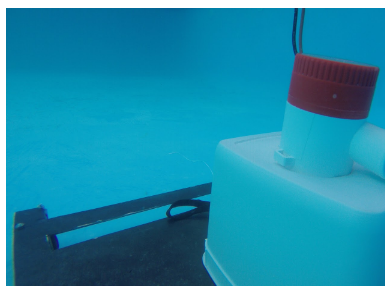
\includegraphics[width=0.6\textwidth]{figures/test.png}
  \caption{Teste de movimentação Robô.}
  \label{fig:test}
\end{figure}
\FloatBarrier
\par

\chapter{Resultados Parciais}
O projeto para construção de um robô capaz de efetuar a limpeza do fundo de piscinas mostrou-se viável e está em desenvolvimento. A estrutura do robô projetada até o momento foi necessária para realização dos testes de movimentação e vedação. Além disso, o desenvolvimento da lógica do robô ao executar o percurso para varrer a piscina, a arquitetura de software e comunicação entre a raspberry pi 2 e o arduino estão implementadas. Os proximos passos serão a conexão do sistema de locomoção, já testado, ao sistema de limpeza e ao sistema de automação. Pretende-se finalizar a estrutura e lógica do robô, bem como realizar testes do seu funcionamento para a próxima entrega.